\section{Proposed Data Structure for Modular Virtual Commissioning} \label{sec:DataStructure}
	Based on the previous chapters, a data structure for a virtual commissioning is presented in this section. The focus lies on the modularity of the individual sub-components of the considered plant. 

\subsection{Modular Structure}
% Modularität
	In order to improve understanding, the data structure is explained with the help of an example. For this purpose, a filling station is considered as part of a larger plant. The design of this station is shown in \autoref{fig:DataStruktureUseLayout} and consists of two identical dosing units (A), a conveyor belt (B) and a separator (C). These sub-components are bought-in parts and are assembled in this station. The product for the customer is the filling station as a complete unit.  \\
	\begin{figure}[htp]
		\centering
		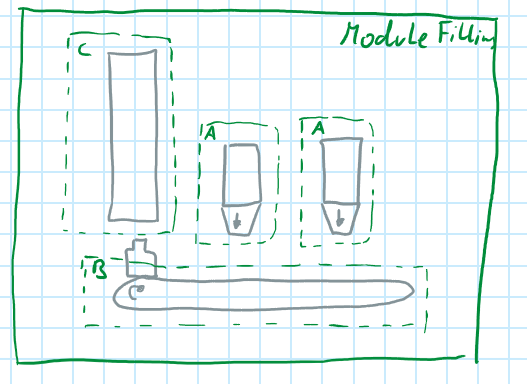
\includegraphics[width=.7\linewidth]{figures/StruktureCad.PNG}
		\caption{Layout of the filling station}
		\label{fig:DataStruktureUseLayout}
	\end{figure}

	The starting point for the development of the filling station are the exchange packages of the three suppliers with the respective product as content. These packages are connected and expanded and finally result in a package with the entire filling station as seen by the customer. In a next step, the customer is able to use the filling station in the planning of the remaining plant. This general procedure is shown in \autoref{fig:DataStruktureComponents}.
	\begin{figure}[htp]
		\centering
		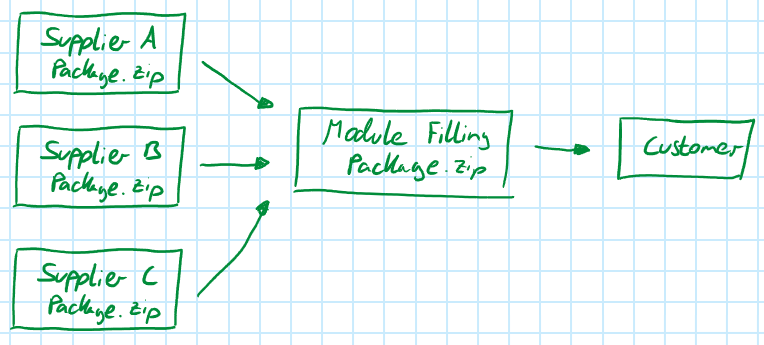
\includegraphics[width=.8\linewidth]{figures/StruktureFile.PNG}
		\caption{File components of the filling station}
		\label{fig:DataStruktureComponents}
	\end{figure}

	% Die tatsächliche Struktur
	The actual setup of the data structure is kept simple and consists of a root folder with several directories for the relevant information as shown in \autoref{fig:DataStruktureHierachry}. This root folder is finally compressed into a \textit{.zip} file for distribution. Due to the plain and simple structure, it can be easily extended and modularly exchanged.  
	\begin{figure}[htp]
		\centering
%		\footnotesize
		\scriptsize
		\tikzstyle{every node}=[draw=black,thick,anchor=west]
		\tikzstyle{basis}=[draw=black,fill=black!10]
		\begin{tikzpicture}[%
			grow via three points={one child at (0.5,-0.7) and
				two children at (0.5,-0.7) and (0.5,-1.4)},
			edge from parent path={(\tikzparentnode.south) |- (\tikzchildnode.west)}]
			\node [basis] {Data Structure}
			child { node {Geometry (CAD)}}		
			child { node {Control Software}}
			child { node {Behaviour Model}}
			child { node {Documentation}}
			child { node {\dots}}			
			child [missing] {}				
			child [missing] {}				
			child [missing] {};
		\end{tikzpicture}
		\caption{Data structure}
		\label{fig:DataStruktureHierachry}
	\end{figure}



\subsection{Used File Formats}
	As already mentioned in \autoref{sec:AvailableDataFormats}, a wide range of possible data formats exists to represent the required information for virtual commissioning. The focus in the selection of the used formats, should be on the widest possible support in different tools. Only through this approach the format can become accepted in the industry. In this section, the formats are selected and the result is summarized in \autoref{tab:InformationAndFormats}. \\

% Beschreibung und Begründung für alle Punkte
\subsubsection{Geometry and CAD}
	For a loss-free exchange of CAD data, the information of the kinematization of the assemblies must be preserved in addition to the raw geometry. As mentioned earlier, this is a big problem in practical use and therefore the \textit{COLLADA} format would be a optimal solution. At the moment, suitable tools for conversion are missing or do not support the current version of \textit{COLLADA} implementing the kinematization. As a result, using the \textit{COLLADA} format is the optimal solution in theory but in practice native CAD formats are the better choice. Which CAD tool and further which format is finally used has to be defined between the customer and supplier. Alternatively, neutral formats like \textit{.step} can be used, but with the disadvantage of missing kinematics. \\
	For example, \textit{Autodesk Inventor} offers a quick way to exchange data via the \textit{Pack and Go} tool \cite{InventorPackAndGo}. In this case, the entire geometry, dependencies and also materials of an assembly are bundled in one file, which also simplifies the exchange. A similar function is also available in \textit{Solidwork} \cite{SolidworksPackAndGo}. It should be noted, that although the two functions have the same name, they are not compatible with each other. \\

\subsubsection{Behaviour Model}
	The modeling of the physical behavior can also be done using various tools. In contrast to CAD data, a neutral and established format for data exchange already exists here: the \textit{FMI}. A growing number of tools support this format, making it a good choice in a modular virtual commissioning process. \\
	In the academic community, but also in industry, \textit{Matlab/Simulink} is often used for modelling. This tool is very popular mainly because of its flexibility, and supports the import and export of \textit{FMI} files in versions 1 and 2. Instructions for the export can be found in \cite{MatlabFmuExport} and for the import in \cite{MatlabFmuImport}. \\

% PLC Code
\subsubsection{PLC Code}
	The exchange of PLC code is almost no problem in practice. This is thanks to the standardization of automation engineering using PLCs, which also describes the possible programming languages and the exchange format as \textit{.xml} files. In addition to the language basis, more complex functions such as function blocks for movements are also part of the standard and thus easily exchangeable. Thanks to the international validity, many manufacturers rely on this standardization and offer converters to and from the \textit{PLCopen} format. \\

% Documentation and Drawings
\subsubsection{Documentation}
\colorbox{yellow}{To be added}


\begin{table}[htp]
	\scriptsize
	\centering
	\caption{Choosen file formats.}
	\begin{tabular}{ll}
		\toprule
		 \multicolumn{1}{c}{Information} & \multicolumn{1}{c}{Choosen File Format}\\
		 \midrule
		 CAD (pure geometry) & \textit{.step}\\
		 CAD (with kinematics) & Native or \textit{COLLADA}  \\
		 Pyhsical Behavior & \textit{FMU}\\
		 & \\
		 PLC Code & \textit{PLCopen} \\
		 & \\
		 Documentation & \textit{.pdf}\\
		 \bottomrule
	\end{tabular}	
	\label{tab:InformationAndFormats}
\end{table}



\section{Advantages and Disadvantages}
\colorbox{yellow}{To be added}


\section{Workflow of the proposed Data Structure}
% Introduction
\colorbox{yellow}{Description for \autoref{fig:GeneralWorkflow}}. 

\begin{figure}[htp]
	\centering
	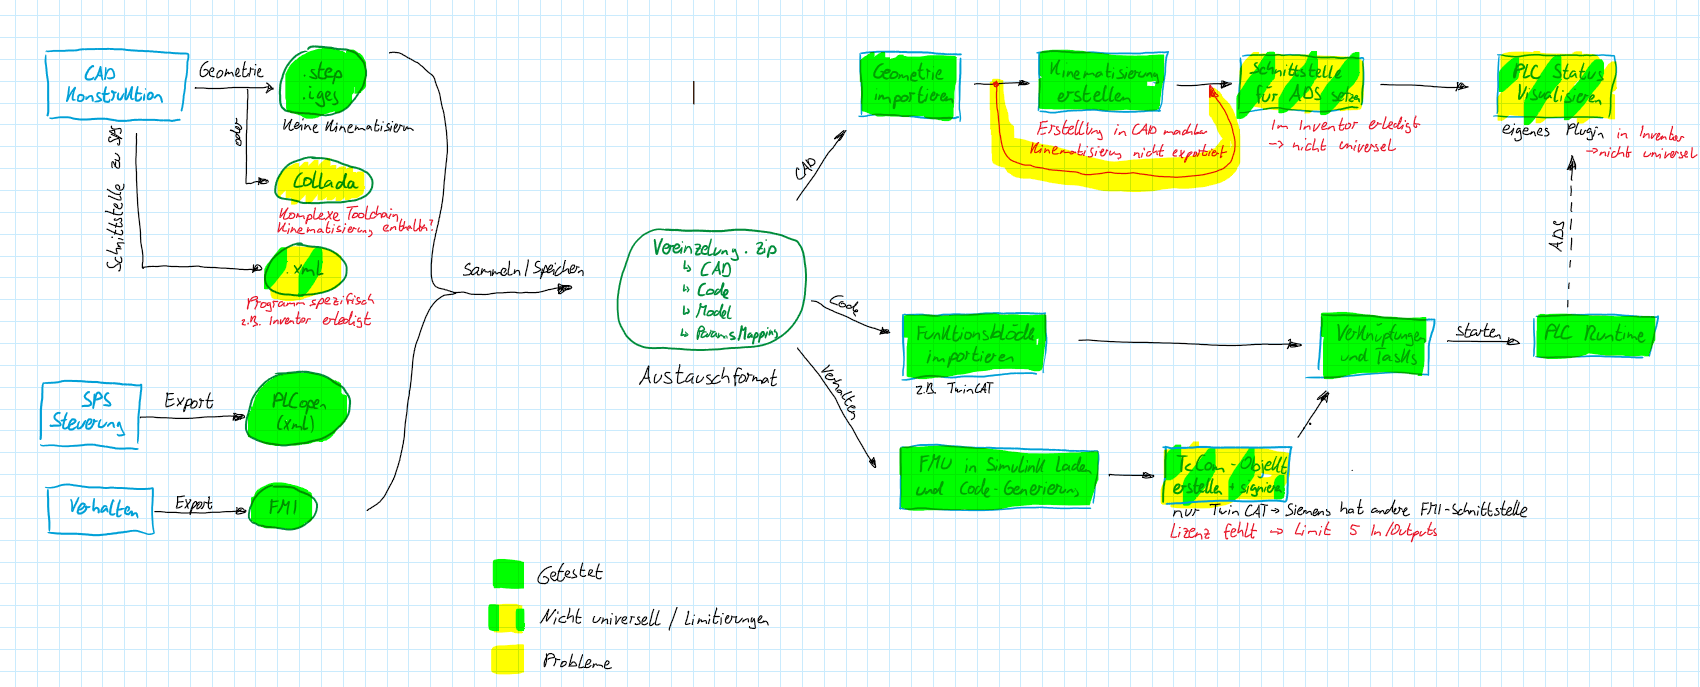
\includegraphics[width=.9\linewidth]{figures/GeneralWorkflow.PNG}
	\caption{General Workflow\colorbox{yellow}{bigger and maybe split into inport and export}}
	\label{fig:GeneralWorkflow}
\end{figure}


